\section{Создание приложения с использованием AngularJS}

После использования фреймворка Backbone.js было решено реализовать приложение с использование с целью выяснения практических преимуществ и недостатков.

Первым делом было решено автоматизировать развертывание приложения и воспользоваться такими средствами как npm и Bower. Npm --- это пакетный менеджер для JavaScript, который является частью проекта Node.js. Этот инструмент позволяет автоматизировать сборку приложения (с использование Bower), тестирование и развертывание. Установка не отличается ничем примечательным --- необходимо из репозиториев или же с официального сайта (http://nodejs.org) произвести установку Node.js и npm идет с ним же\cite{npm}. Все инструкции для автоматизации находятся в файле package.json. В процессе реализации данного приложения был написан следующий файл конфигурации:
\begin{lstlisting}
{
  "name": "adhoc-project",
  "devDependencies": {
    "http-server": "^0.6.1",
    "bower": "^1.3.1"
  },
  "scripts": {
    "postinstall": "bower install",
    "prestart": "npm install",
    "start": "http-server -a 0.0.0.0 -p 8080"
  }
}
\end{lstlisting}

Такая конфигурация позволяет из командой строки выполнить:
\begin{lstlisting}
npm run
\end{lstlisting}

И произойдет следующее: установятся все необходимые зависимости для развертывания приложения, выполнится bower install и запустится веб-сервер на 8080 порту. Таким, образом, не нужно включать в проект зависимые библиотеки --- это произойдет автоматически, основываясь на конфигурации, описанной в package.json.

Для управления зависимостями JavaScript-библиотек был выбран менеджер пакетов Bower. Bower --- не стандартный менеджер пакетов, но самый популярный. Сейчас в репозитории находится более 11 тысяч пакетов\cite{bower}. Bower не навязывает пользователю свою систему сборки, а разработчику пакетов --- метод подключения библиотеки. Всё, что делает Bower --- устанавливает нужные проекту пакеты подходящих версий вместе с их зависимостями. Другими словами: просто загружает файлы нужных библиотек и всё, что нужно для их работы в специальную папку. Остальное остается на усмотрение разработчика.

После установки и настройки npm необходимо настроить конфигурацию Bower. Для этого в каталог проекта необходимо добавить файл bower.json, с содержимым которые напоминает конфигурацию npm:
\begin{lstlisting}
{
  "name": "adhoc-project",
  "private": true,
  "dependencies": {
    "jquery": "",
    "easysoap": "",
    "bootstrap": "3.3.4",
    "angular": "~1.4.0",
    "angular-route": "~1.4.0",
    "angular-resource": "~1.4.0"
  }
}
\end{lstlisting}

\subsection{Структура приложения}

В процессе реализации данного приложения была создана следующая структура каталогов, отображенная на рисунке \ref{angular_structure}. В каталогах \textit{bower\_components} и \textit{node\_modules} хранятся библиотеки, от которых зависит данный проект. Они обновляются автоматически при помощи утилит npm и bower.
\begin{figure}[h]
\center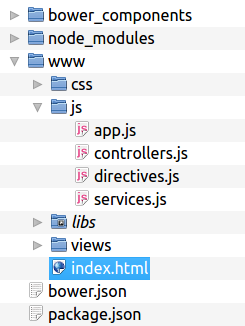
\includegraphics[width=0.4\textwidth]{angular_structure}
\caption{Структура каталогов приложения на AngularJS}\label{angular_structure}
\end{figure}

В каталоге \textit{www} хранится само приложение, где \textit{index.html} --- точка входа приложения. В каталоге \textit{css} находятся таблицы стилей, в каталоге \textit{views} шаблоны представлений. Каталог \textit{libs} представляет собой символическую ссылку на каталог bower\_components и содержит в себе необходимые проекту библиотеки.

При реализации данного проекта потребовались следующие библиотеки:
\begin{enumerate}
 \item jQuery. Библиотека JavaScript, фокусирующаяся на взаимодействии JavaScript и HTML\cite{jquery}.
 \item easySoap. WSDL SOAP клиент для JavaScript.
 \item Twitter Bootstrap. Свободный набор инструментов для создания сайтов и приложений. Включает в себя HTML и CSS шаблоны оформления\cite{bootstrap}.
 \item AngularJS. JavaScript-фреймворк предназначенный для разработки одностраничных приложений на основе MVC шаблона\cite{angular}.
\end{enumerate}

В каталоге \textit{js} находятся четыре JavaScript-скрипта, логически разделенные на различные части приложения: маршрутизация, контроллеры, директивы, сервисы:
\begin{enumerate}
 \item app.js. Описывается структура приложения: используемые модули и маршрутизация.
 \item controllers.js. Модуль, который содержит в себе все контроллеры, определенные в данном проекте.
 \item directives.js. Модуль с реализованными дополнительными директивами: для построения графика и для вывода сообщений.
 \item services.js. Модуль, в котором реализованы различные сервисы для работы с данными: получение/отправка данных на сервис по протоколу SOAP, сервис для обработки сообщений пользователю и сервис для перевода машинных идентификаторов в формат, понятный человеку.
\end{enumerate}
